\chapter{Experimental Methods}
\label{methods}
\section{Protein purification} 
Ase1-GFP, mEGFP or mCherry tagged tau and tau$\Delta$N, Kinesin-1, Kip3 and katanin were expressed and purified as described previously \parencite{HERNANDEZVEGA20172304,Herrmann2018,Mitra2018,NITZSCHE2010247, Janson2007}.

\subsection{Microtubule preparation}
\subsection{Tubulin preparation}
Tubulin was isolated from pig brains and labeled as described previously \parencite{CASTOLDI200383}: Fresh pig brains were cleaned, homogenized in a blender in a ice-cold depolymerization buffer and centrifuged at 29.000 x g for
60 min at 4 ºC. An equal volume of high molarity PIPES supplemented with 1.5 mM ATP and 0.5 mM GTP and of 37 ºC warm glycerol was added to the supernatant to promote microtubule polymerization. The mixture was then incubated for 60 min at 37 ºC prior to centrifugation at 150.000 x g for 30 min at 37 ºC. The microtubule pellet was subsequently depolymerized by resuspension in ice-cold depolymerization buffer and dounced on ice for 10 min, followed by
incubation for 60 min on ice and centrifugation at 70.000 x g for 30 min at 4 ºC. Next, the supernatant containing depolymerized tubulin was diluted in equal
volumes of prewarmed high molarity PIPES and glycerol supplemented with 1.5 mM
ATP and 0.5 mM GTP, incubated for 30 min at 37 ºC to promote microtubule polymerization and subsequently centrifuged at 150.000 x g for 30 min at 37 ºC.
Finally, the microtubule pellet was depolymerized by resuspension in ice-cold BRB80
and dounced on ice for 10 min. After further incubation for 10 min on ice, the solution
was centrifuged at 100.000 x g for 30 min at 4 ºC (SW 41Ti rotor). Tubulin was then aliquotized and flash frozen in liquid nitrogen and stored at -80 ºC for later use. Some of the tubulin was aliquotized in high concentrations for subsequent labeling as described by \cite{HYMAN1991478}. In brief, tubulin labeling involved polymerizing microtubules and incubating these microtubules with fluorescent dye present, and depolymerizing the microtubules again to yield labelled tubulin.
\subsection{Microtubule polymerization}
For preparation of biotinylated microtubules, isolated tubulin was mixed with biotinylated tubulin (Cytoskeleton Inc., T333P) at 50:1 mass ratio. For preparation of labeled microtubules, isolated tubulin was mixed with labeled tubulin. When working with microtubules, it is often desirable to stabilize microtubules, in other words, to prevent microtubule instability. We employed two techniques: i) Polymerizing microtubules under the presence of GMPCPP, a slowly hydrolyzable GTP analogue \parencite{Hyman1992}. ii) Stabilization of microtubules by having paclitaxel present in the buffer \parencite{SCHIFF1979}. GMPCPP-stabilized microtubules were grown using a mixture of 2 $\mu$M tubulin, 1 mM GMPCPP and 4 mM MgCl$_2$ in BRB80 and incubated for 3 hours at 37°C. Paclitaxel-stabilized microtubules were polymerized using a mixture of 1 mM GTP, 4 mM MgCl$_2$ and 5 \% DMSO in BRB80 for 30 minutes and subsequently stabilized by diluting the mixture in BRB80 + 10 µM paclitaxel. In both the GMPCPP and the paclitaxel procedure, the resulting mixture was then spun at 12000 g in a tabletop centrifuge. Finally, the supernatant was discarded, and the pellet was resuspended in 50 $\mu$l BRB80, respectively BRB80 + 10 µM paclitaxel.

\subsection{Sample Preparation}
\label{assayPREP}
To conduct our microscopy, we implemented a procedure which has already been described earlier \parencite{Gell2010a}. It features TIRF microscopy of microfluidic channels which are manufactured as depicted in \autoref{Gell2010a_setup}A. The coverslips used in the process, after a cleaning procedure, were functionalized with dichlorodimethylsilane (DDS) to allow for antibody binding to the surface.
\begin{figure}[htb]
\centering
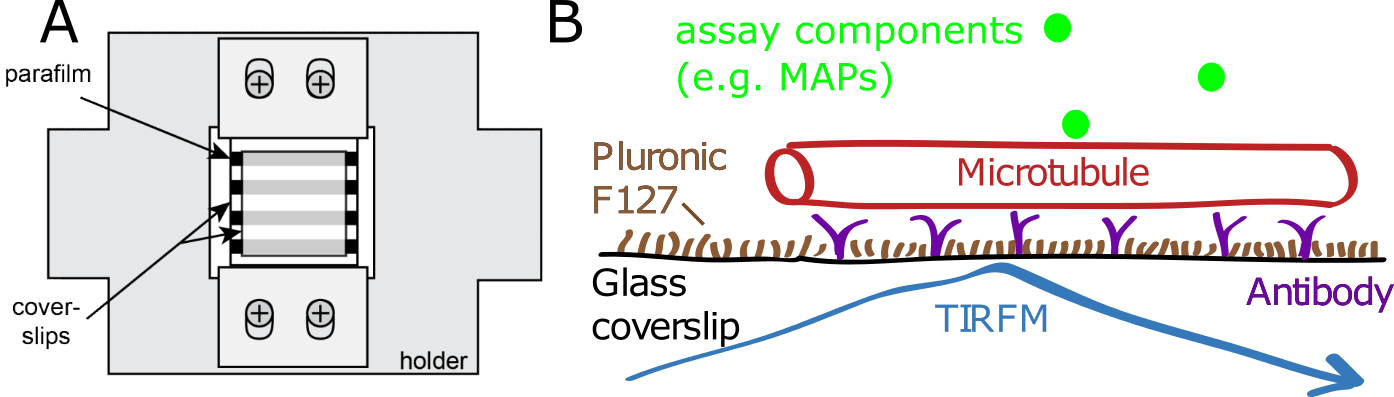
\includegraphics[scale=1.1]{Figures/setup.png}
\caption[The flow cell layout and handling, adapted from \parencite{Gell2010a}]{
		A sketch of the flow cell layout and handling, adapted from \parencite{Gell2010a}. The four depicted Parafilm stripes were put as spacers in between two DDS-coated glass slides to form three channels. To seal the channels, this construct was then heated up for about 30 seconds while gently pressing the upper slide onto the lower. Next, it was clamped into a brass sample holder. To fill the initially dry channels with liquid, vacuum was employed. Further perfusion steps were conducted by simply utilizing a filter paper as is illustrated. \textbf{B} Schematic of our our experimental setup. The labeling of our microtubules and the included assay components varied from experiment to experiment. 
	}\label{Gell2010a_setup}
\end{figure}
After manufacturing, flow channels were incubated with antibodies in PBS for 5 min (to immobilize biotinylated microtubules, we used anti-biotin antibodies, to immobilize microtubules without biotin, we used anti-$\beta$-tubulin antibodies), followed by incubation for at least 30 min with 1\% pluronic F-127 in PBS to prevent unspecific protein binding. The flow channel was then washed with BRB80 prior to addition of microtubules for antibodyspecific binding. Unbound microtubules were then removed in another wash step. After these preparatory steps, the assay buffer was added, and the coverslip holder was mounted onto the microscope stage (setup shown in \autoref{Gell2010a_setup}).

\section{In vitro tau-microtubule binding assay}
Biotinylated, paclitaxel-stabilized, Atto647-labeled microtubules in BRB80T (80 mM Pipes/KOH pH 6.9, 1 mM MgCl2, 1 mM EGTA, 10 µM paclitaxel) were immobilized in a flow chamber using biotin antibodies (Sigma B3640, 20 µg/ml in PBS). Subsequently, the buffer in the flow cell was exchanged for assay buffer (20 mM HEPES pH 7.2, 1 mM EGTA, 75 mM KCl (unless stated otherwise in the main text), 2 mM MgCl2, 1 mM ATP (+Mg), 10 mM dithiothreitol, 0.02 mg/ml casein, 10 µM paclitaxel, 20 mM d-glucose, 0.22 mg/ml glucose oxidase and 20 µg/ml catalase). Then, tau in assay buffer was flushed into the flow cell at the final assay concentration stated in the main text. In experiments including multiple subsequent tau additions, the flow cell was rinsed between each tau addition by high ionic strength buffer (200 mM KCl additional to the assay buffer). To remove tau from solution during experiments presented in Figures 1 and 5, the chamber was perfused with approximately four-fold amount of the chamber volume using assay buffer not containing tau. For high concentrations of tau (>200 nM), higher volumes (up to ten-fold chamber volume) were used to remove tau. In experiments involving kinesin-8, katanin, or kinesin-1, islands were first preformed before the respective protein was added to solution (keeping the tau concentration constant). For the katanin experiment at elevated tau concentration (Figure 6) microtubules were first incubated with 0.8 µM tau-mCherry for 5 minutes. Tau-mCherry was then removed from the measurement chamber for a brief period of time (less then 1 minute) to note the position of the islands (which were obscured by the high tau-mCherry density in the island surroundings). Tau-mCherry was then again added at 0.8 µM. After 5 minutes 215 nM katanin-GFP was added to the solution (while keeping the tau concentration 0.8 µM). All experiments were performed at room temperature. 

\section{In vitro Ase1-microtubule binding assay}
Biotinylated, GMPCPP-stabilized, fluorescence-labeled microtubules in BRB80 (80 mM Pipes/KOH pH 6.9, 1 mM MgCl2, 1 mM EGTA) were immobilized in a flow chamber using biotin antibodies (Sigma B3640, 20 µg ml$_{−1}$ in PBS, setup shown in \autoref{tau1}A). Subsequently, the buffer in the flow cell was exchanged for assay buffer (see below). Then, Ase1 in assay buffer was flushed into the flow cell at the final assay concentration stated in the main text, together with tubulin. Figure TODO experiments were performed at room temperature and with 32$\mu$M unlabeled tubulin present in solution. Figure TODO experiments were performed at 29°C and with 14$\mu$M tubulin, 7\% of which was labeled with rhodamine. The following buffer components common to all used buffers in experiments involving Ase1: 20mM PIPES pH 6.9, 10mM HEPES pH 7.2, 0.5mM EGTA, 1mM MgCl2, 0.5mM Mg-ATP, 0.67mM GTP, 0.67\% Tween20, 6.7mM DTT, 0.3 mg/ml Casein, 13.5mM D-Glucose, 0.3mg/ml glucose oxidase and 0.03mg/ml catalase. The buffer for Figure TODO experiments, in addition to these components, contained 70mM KCl, and 0.1\% Methylcellulose, 0.1\% Glycerol, 1mM sodium phosphate and 1µM ATP. The buffer for Figure TODO experiments, in addition to the components common to all buffers, contained 116mM KCl and 0.065\% Methylcellulose.

\section{Imaging}
Atto647-labeled microtubules, mCherry- and mEGFP-labeled proteins were visualized sequentially by switching between the Cy5, TRITC and GFP channels (Chroma filter-cubes) using Nikon-Ti E microscope equipped with 100x Nikon TIRF objective and either Hamamatsu Orca Flash 4.0 sCMOS or Andor iXon EMCCD cameras.The acquisition rate varied between 1 frame per 30 ms to 1 frame per 30 seconds depending on the particular experiment and is indicated in the corresponding figure.  In the case of assays involving Ase1 as shown in Figures TODO, only the GFP channel was visualized, at a framerate of 5s. For Ase1 experiments as showin in Figures TODO, channels were sequentially switched at a framerate of 2.6 seconds. Imaging conditions in experiments used for quantitative estimation of kinetic parameters were set such that photo-bleaching effects were negligible (< 2 \% fluorescent intensity loss during the experiment). 
\section{Image analysis}
\label{methods_analysis}
Data was analyzed using FIJI \parencite{Schindelin2012} and custom written Matlab (Mathworks) routines. 
\subsection{Density estimation}
Kymographs (KymographBuilder plugin, custom-modified to compute integrated intensity instead of finding the maximum intensity) along the microtubule length were used to read out the fluorescent signal and to estimate the integrated signal intensity of fluorescent proteins bound to the microtubule (if necessary, time series were drift-corrected with FIESTA \parencite{RUHNOW20112820}. The recorded signal in regions directly adjacent to the microtubule was subtracted as background signal. Kymograph pixels were then manually categorized according to the type of microtubule region they covered (island, curved microtubule, regions surrounding the islands in case of tau, overlapping microtubules or single microtubules in the case of Ase1). The integrated intensity averaged along the microtubule length for each region type was then computed for each frame by taking the mean of the categorized kymograph pixels. The density of labeled MAPs bound to the microtubule was then estimated by dividing the averaged integrated intensity by estimated intensity per single molecule times unit length. Conversion to the number of MAP molecules per tubulin dimer (done for tau only) was performed assuming 13 available protofilaments and 8 nm length of a tubulin dimer.

\subsection{Fluorescent signal of a single fluorescent molecule} 
In our assays, we often were interested in the absolute number of labeled proteins bound to microtubules. To estimate this number, it was necessary to know the contribution of single fluorophores to the measured signal. The fluorescent signal of a single fluorescent molecule was determined by generating intensity time-traces of single fluorophore-labeled kinesin-1 molecules tightly bound to the microtubule in presence of AMP-PNP (in the absence of ATP) and estimating the height of the occurring bleaching steps. The number of steps was first estimated by eye, and this number was used as input for the findchangepoints function of Matlab to determine the position of the steps (see \autoref{bleaching_steps}). To yield the intensity per single molecule, the heights of these steps were averaged.
\begin{figure}[htb]
\centering
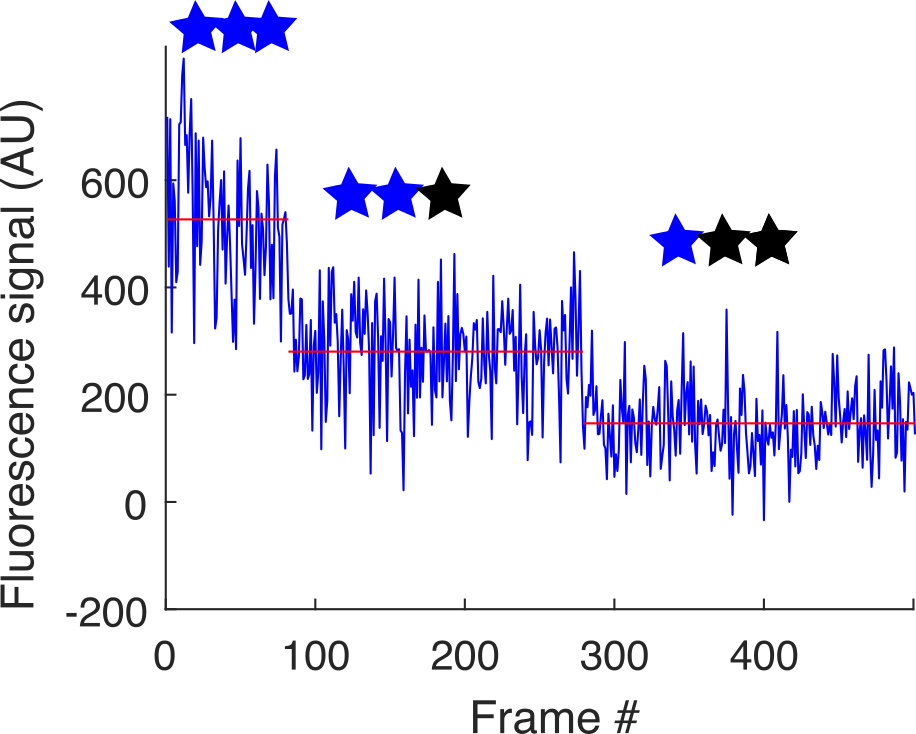
\includegraphics[scale=1.1]{Figures/bleaching_steps.png}
\caption[An illustration explaining our estimation of the fluorescent signal of a single fluorophore.]{
		The signal recorded on a particular spot on a microtubule decorated with immobilized fluorophore-labeled kinesin-1 molecules. The signal shows a step-wise decay due to photobleaching of the fluorophores. The bleaching steps were detected detection of significant changes of the mean values.
	}\label{bleaching_steps}
\end{figure}

\subsection{Procedures specific to tau experiments}
The fraction of microtubule length covered by tau islands has been estimated by approximating islands and microtubules with segmented lines, measuring their lengths and dividing the sum of the lengths of the islands on a single microtubule (or in a field of view) by the length of the respective microtubule on which the islands were located (or by the summed length of all microtubules within a field of view).
\subsubsection{Estimation of the tau unbinding time}
To estimate the unbinding times of tau from inside and outside the islands, we analyzed how the tau density in a given region decayed over time after a buffer exchange either removing tau from solution or replacing tau-mEGFP by tau-mCherry. Every analyzed region (either island or surrounding) yielded a time trace of tau density decay after a buffer exchange. Time-traces from exemplary experiments were combined to be presented in Figures \ref{tau1}F,H and \ref{tau_s1}G  such that the thick line represents the median value of all traces at the given point in time and the bounds represent the first respectively the third quartile. To estimate the mean residence times of tau inside and outside the islands, individual density time-traces as described above were fitted separately by an exponential decay using the Matlab function fit (data points taken before exchange of solution had not been taken into account). The presented fits and mean residence times have been computed by averaging the coefficients of the individual fits.
\subsubsection{Velocity and diffusion coefficient estimation} 
Single tau molecule tracking for the estimation of diffusion coefficient was performed using FIESTA\parencite{RUHNOW20112820} software. For reconnecting tracks, a threshold velocity of 12000 nm/s had been chosen, and tracks were allowed to have at most 3 missing frames between two data points. To minimize false-positive connecting of separate molecules, the tracks obtained by FIESTA were cut into pieces such that the maximum distance between two data points was never above 360 nm. Island boundary assembly and disassembly velocities (in absence or presence of katanin or Kip3) were estimated by approximating straight lines onto segments of advancing or receding tau island edges in kymographs. The value presented in the text is a duration-weighted average of the corresponding segments. Conversion to the number of tau molecules per second was performed by multiplying this velocity by the estimated characteristic tau density within islands (in molecules per nanometer), assuming tau binding to 13 protofilaments and 8 nm length per tubulin dimer. Kip3 and kinesin-1 velocities were estimated by approximating straight lines onto kymographs of moving motors (inside/outside island). 
\subsubsection{Katanin severing rate estimation} 
Severing rates in the areas surrounding the islands were estimated by fitting exponential decay to the number of pixels in the area of the original microtubule position above a threshold value, which was manually set to encompass the microtubule. In island regions, cuts were counted. In Figure \ref{tau6}B, the estimated severing rates include both, straight and curved microtubules. In \ref{tau7}C the severing rates are sorted according to the following definition: straight microtubules were defined as microtubule stretches in which the microtubule orientation would not change beyond 10 degrees; curved regions were defined as 0.5 µm long stretches of microtubule centered at the point of highest curvature with radius < 2.5 µm.

\subsection{Procedures specific to Ase1 experiments}
\subsubsection{Overlap lifetime estimation}
The lifetime of regions of microtubule overlap was estimated for two different configurations: Antiparallel “midzones”, where two dynamic extensions met and formed a dynamic “midzone” (as shown in Figure TODO), and parallel bundles of two dynamic extensions (as shown in Figure TODO). For both antiparallel midzones and parallel bundles, lifetime was taken to start upon the dynamic (GDP) lattices of each involved microtubule being crosslinked (for antiparallel configurations, we additionally required both plus ends to be within 3 microns to each other upon start of the event), and to end upon one of the involved microtubules to shrink back to its GMPCPP-stabilized region. Additionally, for antiparallel bundles the lifetime also ended upon the midzone ceasing to exist. If an overlapping region survived until the end of the recorded time-lapse movie, the event was registered as censored. Figures 1E+F were generated by using the Matlab function ecdf with setting “survival”.

\subsubsection{Microtubule dynamics}
Parameters of microtubule dynamics have been estimated by generating kymographs and approximating the location of microtubule plus ends over time and space with straight lines (for Figure TODO experiments, the Ase1-neon signal was used to visually track microtubule ends, as microtubule were not imaged directly). This directly yielded growth and shrinkage velocities. Rescues were identified as events where a microtubule switches from shrinkage to growth before reaching the GMPCPP-stabilized seed, and catastrophes were events where growth was followed by shrinkage. Rescue and catastrophe rates were estimated by dividing the number of rescues respectively catastrophes by the sum of the total distance shrunk respectively grown by all plus ends.

\subsection{Data representation}
In all boxplots presented in the figures, horizontal midline indicates the median; bottom and top box edges indicate the 25th and 75th percentiles, respectively; the whiskers extend to the most extreme data points not considered as outliers (the function Alternative box plot from the IoSR Matlab Toolbox has been used); the numbers indicate the sample size; the notches are centered on the median and extend to ±1.58*IQR/sqrt(sample size). Where single, colored data points are presented, points from the same experiment are indicated by the same color (unless otherwise stated). 